\documentclass[11pt,a4paper]{report}
\usepackage[textwidth=37em,vmargin=30mm]{geometry}
\usepackage{calc,xunicode,amsmath,amssymb,paralist,enumitem,tabu,booktabs,datetime2,xeCJK,xeCJKfntef,listings}
\usepackage{tocloft,fancyhdr,tcolorbox,xcolor,graphicx,eso-pic,xltxtra,xelatexemoji}

\newcommand{\envyear}[0]{2025}
\newcommand{\envdatestr}[0]{2025-07-27}
\newcommand{\envfinaldir}[0]{webdb/2025/20250727/final}

\usepackage[hidelinks]{hyperref}
\hypersetup{
    colorlinks=false,
    pdfpagemode=FullScreen,
    pdftitle={Web Digest - \envdatestr}
}

\setlength{\cftbeforechapskip}{10pt}
\renewcommand{\cftchapfont}{\rmfamily\bfseries\large\raggedright}
\setlength{\cftbeforesecskip}{2pt}
\renewcommand{\cftsecfont}{\sffamily\small\raggedright}

\setdefaultleftmargin{2em}{2em}{1em}{1em}{1em}{1em}

\usepackage{xeCJK,xeCJKfntef}
\xeCJKsetup{PunctStyle=plain,RubberPunctSkip=false,CJKglue=\strut\hskip 0pt plus 0.1em minus 0.05em,CJKecglue=\strut\hskip 0.22em plus 0.2em}
\XeTeXlinebreaklocale "zh"
\XeTeXlinebreakskip = 0pt


\setmainfont{Brygada 1918}
\setromanfont{Brygada 1918}
\setsansfont{IBM Plex Sans}
\setmonofont{JetBrains Mono NL}
\setCJKmainfont{Noto Serif CJK SC}
\setCJKromanfont{Noto Serif CJK SC}
\setCJKsansfont{Noto Sans CJK SC}
\setCJKmonofont{Noto Sans CJK SC}

\setlength{\parindent}{0pt}
\setlength{\parskip}{8pt}
\linespread{1.15}

\lstset{
	basicstyle=\ttfamily\footnotesize,
	numbersep=5pt,
	backgroundcolor=\color{black!5},
	showspaces=false,
	showstringspaces=false,
	showtabs=false,
	tabsize=2,
	captionpos=b,
	breaklines=true,
	breakatwhitespace=true,
	breakautoindent=true,
	linewidth=\textwidth
}






\newcommand{\coverpic}[2]{
    % argv: itemurl, authorname
    Cover photo by #2~~(\href{#1}{#1})
}
\newcommand{\makeheader}[0]{
    \begin{titlepage}
        % \newgeometry{hmargin=15mm,tmargin=21mm,bmargin=12mm}
        \begin{center}
            
            \rmfamily\scshape
            \fontspec{BaskervilleF}
            \fontspec{Old Standard}
            \fontsize{59pt}{70pt}\selectfont
            WEB\hfill DIGEST
            
            \vfill
            % \vskip 30pt
            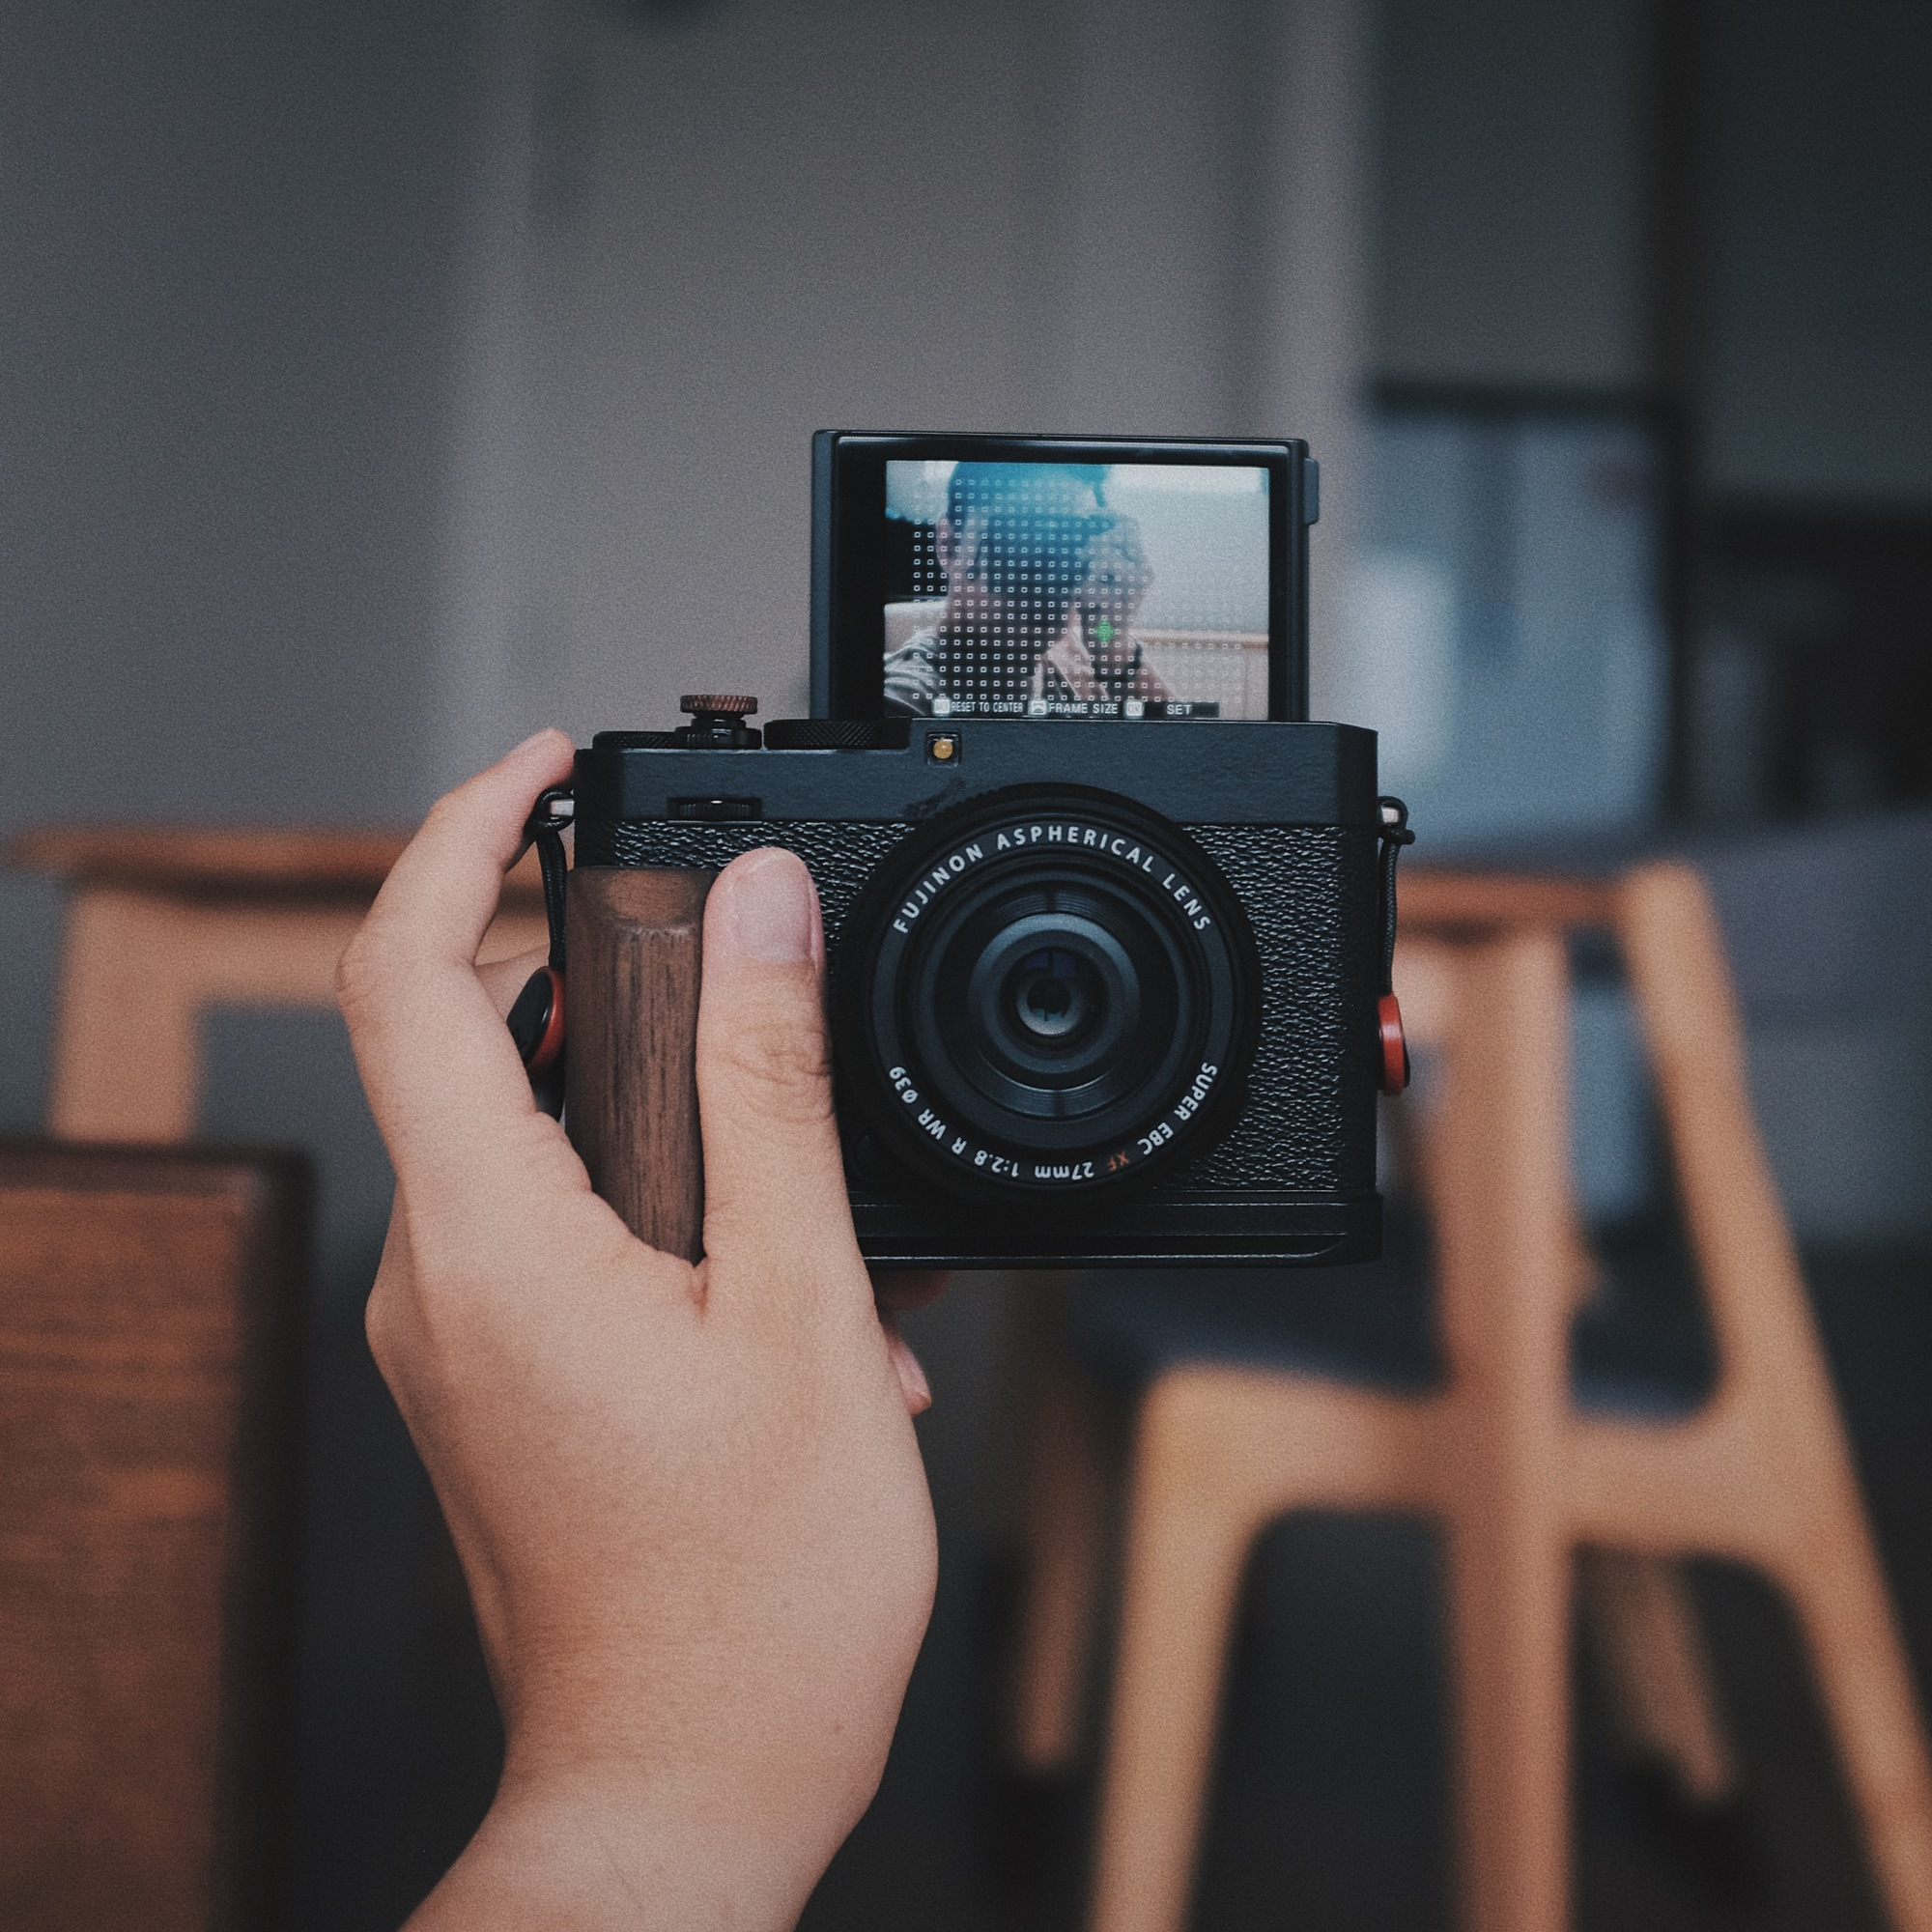
\includegraphics[width=\linewidth]{\envfinaldir/coverpic-prod.jpg}\par
            % \vskip 30pt
            \vfill

            \normalsize\rmfamily\scshape
            \copyright{} The Web Digest Project \hfill\large \envdatestr
        \end{center}
    \end{titlepage}
    % \restoregeometry
}
\newcommand{\simplehref}[1]{%
    \textcolor{blue!80!green}{\href{#1}{#1}}%
}
\renewcommand{\contentsname}{\center\Huge\sffamily\bfseries Contents\par\vskip 20pt}
\newcounter{ipartcounter}
\setcounter{ipartcounter}{0}
\newcommand{\ipart}[1]{
    % \vskip 20pt
    \clearpage
    \stepcounter{ipartcounter}
    \phantomsection
    \addcontentsline{toc}{chapter}{#1}
    % \begin{center}
    %     \Huge
    %     \sffamily\bfseries
    %     #1
    % \end{center}
    % \vskip 20pt plus 7pt
}
\newcounter{ichaptercounter}
\setcounter{ichaptercounter}{0}
\newcommand{\ichapter}[1]{
    % \vskip 20pt
    \clearpage
    \stepcounter{ichaptercounter}
    \phantomsection
    \addcontentsline{toc}{section}{\numberline{\arabic{ichaptercounter}}#1}
    \begin{center}
        \Huge
        \sffamily\bfseries
        #1
    \end{center}
    \vskip 20pt plus 7pt
}
\newcommand{\entrytitlefont}[1]{\subsection*{\raggedright\Large\sffamily\bfseries#1}}
\newcommand{\entryitemGeneric}[2]{
    % argv: title, url
    \parbox{\linewidth}{
        \entrytitlefont{#1}\par\vskip 5pt
        \footnotesize\ttfamily\mdseries
        \simplehref{#2}
    }\vskip 11pt plus 11pt minus 1pt
}
\newcommand{\entryitemGithub}[3]{
    % argv: title, url, desc
    \parbox{\linewidth}{
        \entrytitlefont{#1}\par\vskip 5pt
        \footnotesize\ttfamily\mdseries
        \simplehref{#2}\par\vskip 5pt
        \small\rmfamily\mdseries#3
    }\vskip 11pt plus 11pt minus 1pt
}
\newcommand{\entryitemAp}[3]{
    % argv: title, url, desc
    \parbox{\linewidth}{
        \entrytitlefont{#1}\par\vskip 5pt
        \footnotesize\ttfamily\mdseries
        \simplehref{#2}\par\vskip 5pt
        \small\rmfamily\mdseries#3
    }\vskip 11pt plus 11pt minus 1pt
}
\newcommand{\entryitemHackernews}[3]{
    % argv: title, hnurl, rawurl
    % \parbox{\linewidth}{
    %     \entrytitlefont{#1}\par\vskip 5pt
    %     \footnotesize\ttfamily\mdseries
    %     \simplehref{#3}\par
    %     \textcolor{black!50}{\href{#2}{#2}}
    % }\vskip 11pt plus 11pt minus 1pt
    \begin{minipage}{\linewidth}
            \entrytitlefont{#1}\par\vskip 5pt
            \footnotesize\ttfamily\mdseries
            \simplehref{#3}\par
            \textcolor{black!50}{\href{#2}{#2}}
    \end{minipage}\par\vskip 11pt plus 11pt minus 1pt
}







\begin{document}

\makeheader

\tableofcontents\clearpage




\ipart{Developers}
\ichapter{Hacker News}
\entryitemTwoLinks{Test Results for AMD Zen 5}{https://news.ycombinator.com/item?id=44696167}{https://www.agner.org/forum/viewtopic.php?t=287\&start=10}

\entryitemTwoLinks{Earth Has Tilted 31.5 Inches. That Shouldn't Happen}{https://news.ycombinator.com/item?id=44695205}{https://www.popularmechanics.com/science/environment/a65515974/why-earth-has-tilted-science/}

\entryitemTwoLinks{Ageing accelerates around age 50 ― some organs faster than others}{https://news.ycombinator.com/item?id=44695190}{https://www.nature.com/articles/d41586-025-02333-z}

\entryitemTwoLinks{How We Rooted Copilot}{https://news.ycombinator.com/item?id=44695098}{https://research.eye.security/how-we-rooted-copilot/}

\entryitemTwoLinks{The natural diamond industry is getting rocked. Thank the lab-grown variety}{https://news.ycombinator.com/item?id=44693570}{https://www.cbc.ca/news/business/lab-grown-diamonds-1.7592336}

\entryitemTwoLinks{Bringing a decade old bicycle navigator back to life with open source software}{https://news.ycombinator.com/item?id=44693129}{https://raymii.org/s/blog/Bringing\_a\_Decade\_Old\_Bicycle\_Navigator\_Back\_to\_Life\_with\_Open\_Source\_Software\_and\_DOOM.html}

\entryitemTwoLinks{Rust running on every GPU}{https://news.ycombinator.com/item?id=44692876}{https://rust-gpu.github.io/blog/2025/07/25/rust-on-every-gpu/}

\entryitemTwoLinks{Simon Tatham's Portable Puzzle Collection}{https://news.ycombinator.com/item?id=44691935}{https://www.chiark.greenend.org.uk/~sgtatham/puzzles/}

\entryitemTwoLinks{Users claim Discord's age verification can be tricked with video game characters}{https://news.ycombinator.com/item?id=44691312}{https://www.thepinknews.com/2025/07/25/discord-video-game-characters-age-verification-checks-uk-online-safety-act/}

\entryitemTwoLinks{CCTV footage captures video of an earthquake fault in motion}{https://news.ycombinator.com/item?id=44690911}{https://www.smithsonianmag.com/smart-news/cctv-footage-captures-the-first-ever-video-of-an-earthquake-fault-in-motion-shining-a-rare-light-on-seismic-dynamics-180987034/}

\entryitemTwoLinks{Do not download the app, use the website}{https://news.ycombinator.com/item?id=44689059}{https://idiallo.com/blog/dont-download-apps}

\entryitemTwoLinks{Immigration agents told a teenage US citizen: 'You've got no rights.'}{https://news.ycombinator.com/item?id=44688673}{https://www.theguardian.com/us-news/2025/jul/25/florida-teen-immigration-arrest}

\entryitemTwoLinks{It's time for modern CSS to kill the SPA}{https://news.ycombinator.com/item?id=44688489}{https://www.jonoalderson.com/conjecture/its-time-for-modern-css-to-kill-the-spa/}

\entryitemTwoLinks{Experimental surgery performed by AI-driven surgical robot}{https://news.ycombinator.com/item?id=44688096}{https://arstechnica.com/science/2025/07/experimental-surgery-performed-by-ai-driven-surgical-robot/}

\entryitemTwoLinks{Claude Code introduces specialized sub-agents}{https://news.ycombinator.com/item?id=44686726}{https://docs.anthropic.com/en/docs/claude-code/sub-agents}

\entryitemTwoLinks{Vanilla JavaScript support for Tailwind Plus}{https://news.ycombinator.com/item?id=44686317}{https://tailwindcss.com/blog/vanilla-js-support-for-tailwind-plus}

\entryitemTwoLinks{The Tabs vs. Spaces war is over, and spaces have emerged victorious}{https://news.ycombinator.com/item?id=44686209}{https://xn--gckvb8fzb.com/tabs-vs-spaces-the-war-is-over/}

\entryitemTwoLinks{Animated Cursors}{https://news.ycombinator.com/item?id=44686164}{https://tattoy.sh/news/animated-cursors/}

\entryitemTwoLinks{Never write your own date parsing library}{https://news.ycombinator.com/item?id=44685875}{https://www.zachleat.com/web/adventures-in-date-parsing/}

\entryitemTwoLinks{Internet Archive is now a federal depository library}{https://news.ycombinator.com/item?id=44685342}{https://www.kqed.org/news/12049420/sf-based-internet-archive-is-now-a-federal-depository-library-what-does-that-mean}


\ipart{Developers~~~~(zh-Hans)}
\ichapter{Solidot}
\entryitemGeneric{\hskip 0pt{}Wayback 0.1 释出}{https://www.solidot.org/story?sid=81894}

\entryitemGeneric{\hskip 0pt{}AMD CEO 称台积电美国工厂制造的芯片贵 5\%-20\%}{https://www.solidot.org/story?sid=81893}

\entryitemGeneric{\hskip 0pt{}微软 CEO 轻淡的回应公司裁员之谜}{https://www.solidot.org/story?sid=81892}

\entryitemGeneric{\hskip 0pt{}Mistral AI 环境报告证实 AI 是一个饥渴的怪物}{https://www.solidot.org/story?sid=81891}

\entryitemGeneric{\hskip 0pt{}特朗普威胁关闭 TikTok }{https://www.solidot.org/story?sid=81890}

\entryitemGeneric{\hskip 0pt{}Debian 13.0 Trixie 的新变化}{https://www.solidot.org/story?sid=81889}

\entryitemGeneric{\hskip 0pt{}GPD 推出配备 Ryzen AI Max+ 395 的掌机}{https://www.solidot.org/story?sid=81888}

\entryitemGeneric{\hskip 0pt{}日本将允许用 iPS 细胞制造人类受精卵}{https://www.solidot.org/story?sid=81887}

\entryitemGeneric{\hskip 0pt{}英特尔今年将裁员 2.4 万人}{https://www.solidot.org/story?sid=81886}

\entryitemGeneric{\hskip 0pt{}2023 年的海洋热浪史无前例}{https://www.solidot.org/story?sid=81885}

\entryitemGeneric{\hskip 0pt{}CERN 演示反物质量子比特}{https://www.solidot.org/story?sid=81884}

\entryitemGeneric{\hskip 0pt{}国际法院认为健康环境是人权}{https://www.solidot.org/story?sid=81883}

\entryitemGeneric{\hskip 0pt{}Telegram 上的偷拍群组}{https://www.solidot.org/story?sid=81882}

\entryitemGeneric{\hskip 0pt{}FDA 的 AI 工具被发现捏造研究}{https://www.solidot.org/story?sid=81881}

\entryitemGeneric{\hskip 0pt{}硅谷 AI 创业公司拥抱中国的 996 工作制}{https://www.solidot.org/story?sid=81880}

\entryitemGeneric{\hskip 0pt{}图瓦卢逾八成国民寻求澳大利亚的气候移民签证}{https://www.solidot.org/story?sid=81879}

\entryitemGeneric{\hskip 0pt{}索尼通过降低 PS5 性能应对全球气候变化}{https://www.solidot.org/story?sid=81877}

\entryitemGeneric{\hskip 0pt{}AWS 关闭上海 AI 研究中心}{https://www.solidot.org/story?sid=81876}

\entryitemGeneric{\hskip 0pt{}英国将禁止公共部门向勒索软件组织支付赎金}{https://www.solidot.org/story?sid=81875}

\entryitemGeneric{\hskip 0pt{}Steam 之后 Itch.io 限制成人游戏}{https://www.solidot.org/story?sid=81874}\ichapter{V2EX}
\entryitemGeneric{\hskip 0pt{}[问与答] ai 时代 有什么好的记账软件推荐一下}{https://www.v2ex.com/t/1147938}

\entryitemGeneric{\hskip 0pt{}[问与答] c\#如何使用 winring0.sys 读写 EC 嵌入式控制器}{https://www.v2ex.com/t/1147937}

\entryitemGeneric{\hskip 0pt{}[职场话题] 上家领了大礼包离职的,找工作 HR 面如何说自己的离职原因?}{https://www.v2ex.com/t/1147936}

\entryitemGeneric{\hskip 0pt{}[程序员] 求解答 百度网盘 下载券 原理}{https://www.v2ex.com/t/1147935}

\entryitemGeneric{\hskip 0pt{}[分享创造] 自建了一个 V2EX 新帖推送频道}{https://www.v2ex.com/t/1147934}

\entryitemGeneric{\hskip 0pt{}[分享创造] ChatFlex——让 AI 对话回归简单}{https://www.v2ex.com/t/1147933}

\entryitemGeneric{\hskip 0pt{}[程序员] 倒反天罡 ,我用 Claude Code 搭建了一个 Claude Code 的镜像站~~}{https://www.v2ex.com/t/1147932}

\entryitemGeneric{\hskip 0pt{}[问与答] 求助一下,有没有用 vscode 开发 unity,语言服务器问题}{https://www.v2ex.com/t/1147931}

\entryitemGeneric{\hskip 0pt{}[信息安全] 华为账号一键登录的服务在哪可以取消?}{https://www.v2ex.com/t/1147930}

\entryitemGeneric{\hskip 0pt{}[Solana] V 币不是空气币——V2EX 币的经济学分析}{https://www.v2ex.com/t/1147929}

\entryitemGeneric{\hskip 0pt{}[NAS] 成品 X86 NAS 主机求推荐}{https://www.v2ex.com/t/1147928}

\entryitemGeneric{\hskip 0pt{}[PHP] laravel 和 thinkphp 选择哪个?}{https://www.v2ex.com/t/1147927}

\entryitemGeneric{\hskip 0pt{}[分享发现] 推荐一个小众音乐平台}{https://www.v2ex.com/t/1147926}

\entryitemGeneric{\hskip 0pt{}[加密货币] 庞氏? usdt 32\%APR}{https://www.v2ex.com/t/1147925}

\entryitemGeneric{\hskip 0pt{}[职场话题] 劳动者离职时,用人单位针对离职人员在离职后的 15 日内变更社保减员信息时,在北京人社系统中填写并选择``个人停止缴费原因'',是以下这些选项吗?}{https://www.v2ex.com/t/1147924}

\entryitemGeneric{\hskip 0pt{}[问与答] V 友的 AI 王炸组合🧨🧨🧨🧨}{https://www.v2ex.com/t/1147923}

\entryitemGeneric{\hskip 0pt{}[Claude] 用 Claude Code 做了个 Claude Code 的成本计算器}{https://www.v2ex.com/t/1147922}

\entryitemGeneric{\hskip 0pt{}[ WATCH] 为什么一觉睡醒会显示有一百多的步数}{https://www.v2ex.com/t/1147921}

\entryitemGeneric{\hskip 0pt{}[Solana] 一个方便买 sol 和 V2EX 的方法}{https://www.v2ex.com/t/1147919}

\entryitemGeneric{\hskip 0pt{}[程序员] 字节开源了其智能体开发平台 coze}{https://www.v2ex.com/t/1147917}

\entryitemGeneric{\hskip 0pt{}[程序员] 如今 ai 很火,请教一下大佬们, v 友们是在哪些平台查看最新最火的 ai 趋势,工具🔧?}{https://www.v2ex.com/t/1147916}

\entryitemGeneric{\hskip 0pt{}[酷工作] [惠州-上海闵行] 上位机总工程师 (2-4 年)}{https://www.v2ex.com/t/1147915}

\entryitemGeneric{\hskip 0pt{}[智能家电] 有哪些电池供电、长续航、提供 GPIO 口、可编程的无线超低功耗传感器?}{https://www.v2ex.com/t/1147914}

\entryitemGeneric{\hskip 0pt{}[Windows] WIN11 更新弹窗退退退}{https://www.v2ex.com/t/1147912}

\entryitemGeneric{\hskip 0pt{}[Solana] V2EX, sol 中国最大的社区!}{https://www.v2ex.com/t/1147911}

\entryitemGeneric{\hskip 0pt{}[YubiKey] 请问 yubikey 到底用着怎么样?目前有什么平替吗?}{https://www.v2ex.com/t/1147910}

\entryitemGeneric{\hskip 0pt{}[推广] 亚马逊中国区 3 折 天翼云 45 折~}{https://www.v2ex.com/t/1147909}

\entryitemGeneric{\hskip 0pt{}[问与答] 为啥果味无尼古丁的电子烟能轻易代替传统香烟?}{https://www.v2ex.com/t/1147908}

\entryitemGeneric{\hskip 0pt{}[Tesla] Tesla 后排怎样改善乘坐舒适度?}{https://www.v2ex.com/t/1147906}

\entryitemGeneric{\hskip 0pt{}[Solana] 评论过 k 显示格式问题}{https://www.v2ex.com/t/1147905}

\entryitemGeneric{\hskip 0pt{}[Solana] 一天的买币之旅}{https://www.v2ex.com/t/1147904}

\entryitemGeneric{\hskip 0pt{}[生活] 第一次按摩感觉真酸爽}{https://www.v2ex.com/t/1147903}

\entryitemGeneric{\hskip 0pt{}[Linux] CentOS Stream 对比 CentOS 的变化就是没有小版本号以及先于 RHEL 发布吧?}{https://www.v2ex.com/t/1147902}

\entryitemGeneric{\hskip 0pt{}[职场话题] 在软件开发领域, AI 会有能力边界吗?}{https://www.v2ex.com/t/1147901}

\entryitemGeneric{\hskip 0pt{}[分享发现] 为 V2EX 接口做了 OpenAPI 及 Apifox 格式的文档}{https://www.v2ex.com/t/1147900}

\entryitemGeneric{\hskip 0pt{}[健康] 开始断食辟谷了。空腹已 48 小时。。}{https://www.v2ex.com/t/1147898}

\entryitemGeneric{\hskip 0pt{}[macOS] mac 连接蓝牙鼠标的时候,每次鼠标从关闭改为打开,就连不上了,得重新配对}{https://www.v2ex.com/t/1147897}

\entryitemGeneric{\hskip 0pt{}[云计算] 因华为云业务策略调整,计划于 2025 年 7 月 26 日 17:00(北京时间)正式停售域名注册服务 Domains。}{https://www.v2ex.com/t/1147896}

\entryitemGeneric{\hskip 0pt{}[分享发现] 我是不是最后一个知道淘宝上还能点外卖的?}{https://www.v2ex.com/t/1147895}

\entryitemGeneric{\hskip 0pt{}[Solana] 在 Glow app 里 stake 了 Solana,显示 activating,一直没收益}{https://www.v2ex.com/t/1147894}

\entryitemGeneric{\hskip 0pt{}[Telegram] 为什么 Telegram 桌面端更新可以如此丝滑?}{https://www.v2ex.com/t/1147891}

\entryitemGeneric{\hskip 0pt{}[Apple] 家里的 MacMini 5900 端口被扫,挂在了一个 VNC 公开网站上}{https://www.v2ex.com/t/1147890}

\entryitemGeneric{\hskip 0pt{}[Steam] Steamdeck 充电头被孩子搞坏了}{https://www.v2ex.com/t/1147888}

\entryitemGeneric{\hskip 0pt{}[分享发现] Color Visited - 已访问链接染色脚本}{https://www.v2ex.com/t/1147887}

\entryitemGeneric{\hskip 0pt{}[Solana] Solana 钱包注册的账号如何设置密码?}{https://www.v2ex.com/t/1147886}

\entryitemGeneric{\hskip 0pt{}[健康] 开始辟谷了。空腹已 48 小时。准备空腹一周}{https://www.v2ex.com/t/1147885}

\entryitemGeneric{\hskip 0pt{}[程序员] 非英文技术语言简中最多是错觉吗}{https://www.v2ex.com/t/1147883}

\entryitemGeneric{\hskip 0pt{}[问与答] 新开店铺甲醛不会超标吗}{https://www.v2ex.com/t/1147882}

\entryitemGeneric{\hskip 0pt{}[分享创造] 烧了一万多块,尝试让 AI 写一千篇有趣的内容}{https://www.v2ex.com/t/1147881}

\entryitemGeneric{\hskip 0pt{}[随想] AI 如何杀死人类?}{https://www.v2ex.com/t/1147880}


\ipart{Generic News}







\clearpage
\leavevmode\vfill
\footnotesize

Copyright \copyright{} 2023-2025 Neruthes and other contributors.

This document is published with CC BY-NC-ND 4.0 license.

The entries listed in this newsletter may be copyrighted by their respective creators.

This newsletter is generated by the Web Digest project.

The newsletters are also delivered via Telegram channel \CJKunderline{\href{https://t.me/webdigestchannel}{https://t.me/webdigestchannel}}.\\
RSS feed is available at \CJKunderline{\href{https://webdigest.pages.dev/rss.xml}{https://webdigest.pages.dev/rss.xml}}.

This newsletter is available in PDF at
\CJKunderline{\href{https://webdigest.pages.dev/}{https://webdigest.pages.dev/}}.

The source code being used to generate this newsletter is available at\\
\CJKunderline{\href{https://github.com/neruthes/webdigest}{https://github.com/neruthes/webdigest}}.

This newsletter is also available in
\CJKunderline{\href{http://webdigest.pages.dev/readhtml/\envyear/WebDigest-20250727.html}{HTML}} and
\CJKunderline{\href{https://github.com/neruthes/webdigest/blob/master/markdown/\envyear/WebDigest-20250727.md}{Markdown}}.


\coverpic{https://unsplash.com/photos/people-walk-past-a-yellow-building-on-a-sunny-day-2EWHqTelyMw}{Richard Stachmann}


\end{document}
